\part{The language}\label{part:zilch}

\chapter{Introduction}\label{chap:zilch-introduction}

Low-level programming is programming with a few abstractions over the hardware.
For example, assembly languages mostly provide no or very little abstractions over CPU instructions (having one instruction set per target).
Functional programming is a kind of programming focused around functions and their composition.
However, because of this, many functional programming languages have a tendancy to be quite slow, at least compared to ``ordinary'' imperative programming languages.

\href{http://www.ats-lang.org/}{ATS} is one of those programming languages claiming to be both functional and quite low-level.
It compiles to C (therefore has a free FFI), has a complex dependent type system and many other things making it kind of great.
But ATS is hard to learn, because it has so much stuff\ldots

Yet Zilch is also a low-level functional programming language.
But the goal is to design a not-so-hard to learn programming language, while still having strong guarantees about the code written\footnote{When this was written, Zilch was far from production-ready, so most
	of the guarantees have not yet been described here.}.
Prior knowledge about ML-style programming is still recommended before trying to tackle Zilch, but anybody without this kind of knowledge should also be able to learn Zilch fairly easily.

This part will try to describe and formalize (at least a bit, but some parts may be left informal) the Zilch programming language, going from the usual syntax onto the operational semantics.
Implementation details (such as error messages, program optimisations, \ldots) will not be covered by this document.

\section*{Some notes on the notation used}\label{sec:zilch-introduction-notation}

Zilch is really not a small programming language.
Because of that, sometimes we need some specific notation to described things like inference rules.

The mainly used notation is described here, but not necessarily everything will be described (sometimes, a little bit of common sense helps to understand).

\begin{itemize}
	\item Grammar
	      \begin{figure}[H]
		      \centering
		      \scalebox{.5}{
			      \includegraphics{grammar-template-2}
		      }
	      \end{figure}
	      \begin{itemize}
		      \item Sharp rectangles describe that another rule is to be used there (the name of the rule is given in the rectangle);
		      \item Rounded rectangles describe terminal tokens, i.e.\ pieces of string that must be litterally matched;
		      \item The name of the grammar rule defined is given in the top-left corner of the diagram.
		            A rule matches if and only if it is possible to go from the left to the right, only following the rails;
	      \end{itemize}
	\item Type inference rules
	      \begin{itemize}
		      \item $\Gamma$ is the context containing all type-level information such as types of expressions;
		      \item $\Delta$ is the context containing all kind-level information such as types of types;
		      \item The typing judgment $\Delta \Vdash \tau : \kappa$ is used to indicate that the type $\tau$ as the kind $\kappa$ given information in the $\Delta$ context;
		      \item The typing judgment $\Gamma;\Delta \vdash e : \tau \vert \epsilon$ means that $e$ has type $\tau$ in the context $\Gamma, \Delta$ and that evaluating it may yield effects in $\epsilon$;
	      \end{itemize}
\end{itemize}

\chapter{Grammar of Zilch programs}\label{chap:zilch-grammar}

A Zilch program is comprised of three different levels, each included in the next one:
\begin{itemize}
	\item The expression level, where an expression denotes a value which has a statically determined type;
	\item The declaration level, containing all function definitions, type definitions, etc;
	\item The module level, where imports and module declarations live in;
\end{itemize}

\noindent Because it is not easy to materialize indentation properties in the grammar, it will instead be marked using the non-terminals\footnote{Those symbols are reserved and actually used as terminals, so we put them as non-terminals to remove any ambiguity opportunities.} \texttt{\{}, \texttt{\}} and \texttt{;}.
Note that these are not actually present in the source code, and are only a mean of hinting an indentation change.
\texttt{x \{ y; z \}} really means \texttt{x} followed by \texttt{y} which may be more indented or on the same line, and \texttt{z} which must be aligned with the beginning of \texttt{y}.
It therefore describes both layouts:

\noindent\begin{minted}{\zilchlexer}
  -- `y` on the same line as `x`:
  x y
    z
  -- or `y` on a new line:
  x
    y
    z
\end{minted}
\vspace*{\baselineskip}

If you are willing to make your own Zilch compiler, please note that you may also (or only) support the alternative layout as described in grammar rules, by making use of \verb|{|, \verb|;| and \verb|}| as terminals.
It is not recommended, as \verb|;| is \textit{not} a reserved word, but may be considered for simplicity's sake.
It is also not recommended as using \verb|{| and \verb|}| may clash with inline records and implicit parameters.

\section{Lexicon}\label{sec:zilch-grammar-lexical}

This section describes the lexical structure of any Zilch program.
Note that the Unicode alternative syntax does not need to be supported, but makes the code look nicer.

\subsection{Identifiers, operators and reserved words}\label{subsec:zilch-grammar-lexical-identifiers}

Identifiers and operators are composed of only printable characters which are not considered special, and must not form keywords.
Lexically distinguishing between both types of symbols is done by only allowing alphanumeraical characters in identifiers, and symbolic characters in operators.

\begin{figure}[H]
	\centering

	\framebox[\textwidth][c]{
		\parbox{\textwidth}{
			\centering

			\scalebox{.5}{
				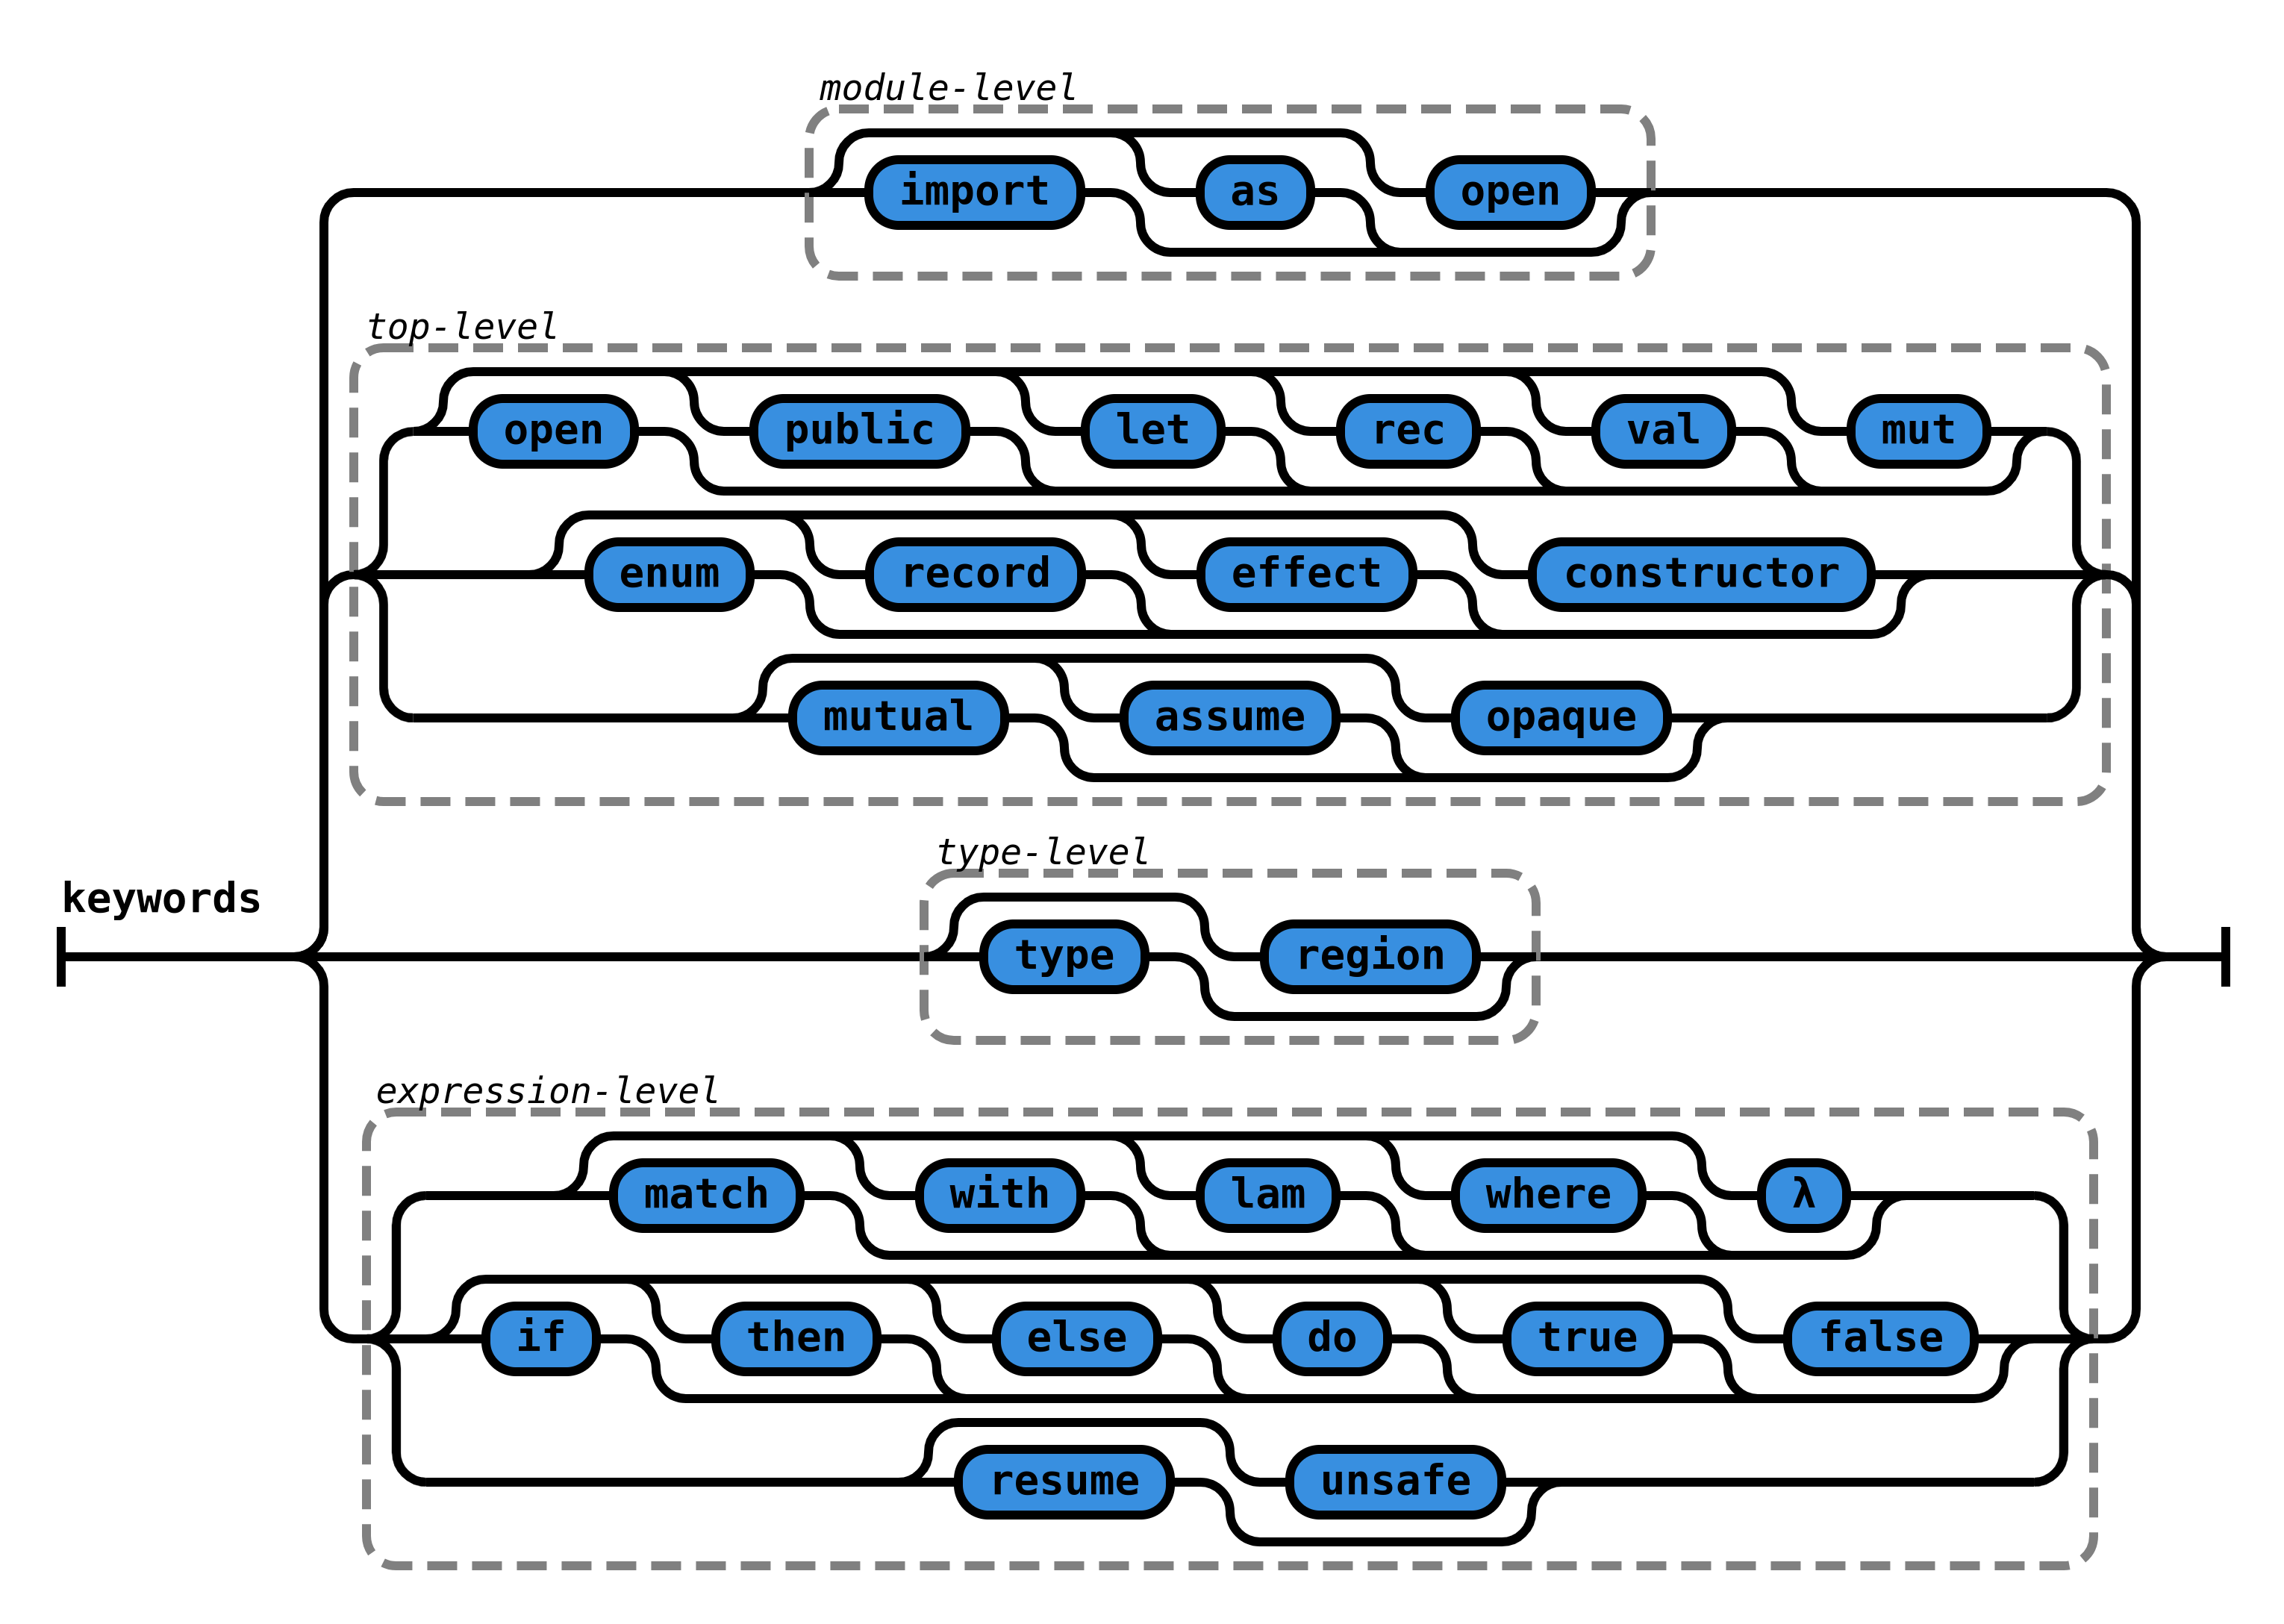
\includegraphics{zilch/lexicon/keywords}
			}
			\\
			\scalebox{.5}{
				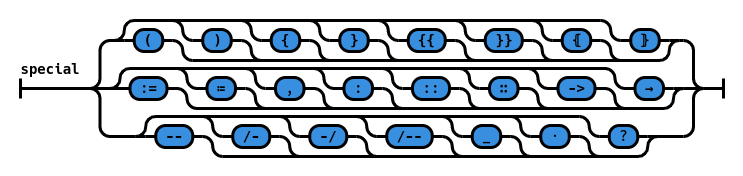
\includegraphics{zilch/lexicon/special}
			}
			\\
			\scalebox{.45}{
				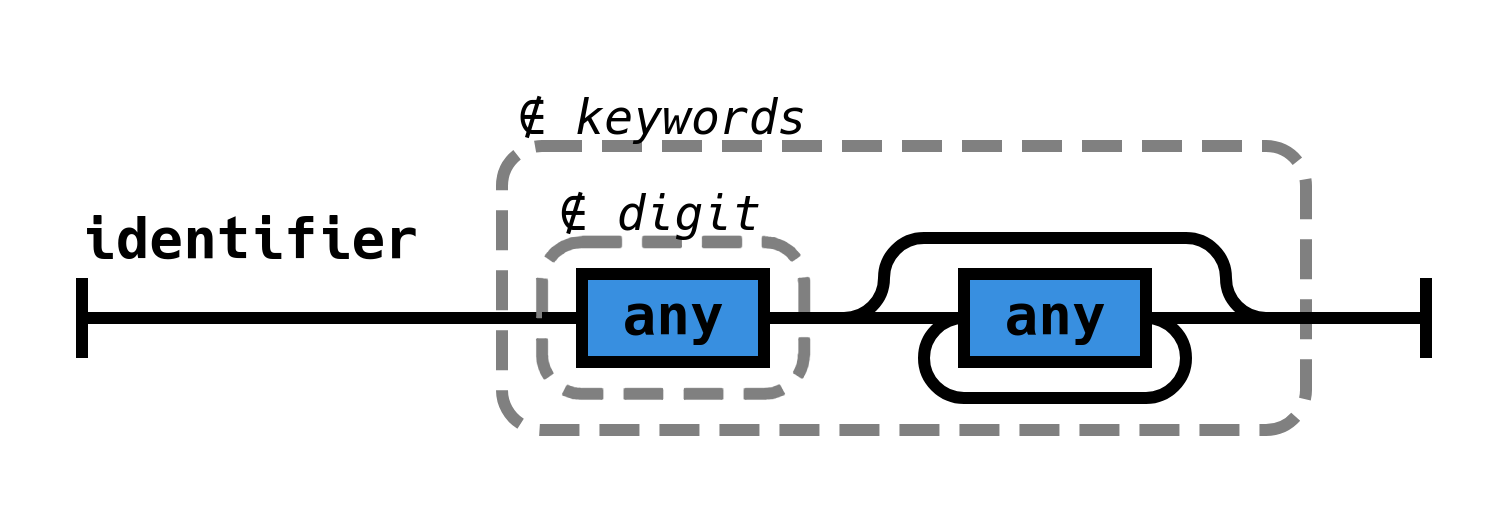
\includegraphics{zilch/lexicon/identifier}
			}
			\scalebox{.45}{
				\includegraphics{zilch/lexicon/symbol}
			}
		}
	}

	\caption{Lexical units for identifiers and operators.}
	\label{fig:zilch-grammar-lexical-identifiers-grammar}
\end{figure}

\subsection{Whitespaces}\label{subsec:zilch-grammar-lexical-whitespaces}

Whitespace tokens are basically word separators.
Because of that, comments are also counted as whitespaces, despite not really being an invisible sequence.

\begin{figure}[H]
	\centering

	\framebox[\textwidth][c]{
		\scalebox{.5}{
			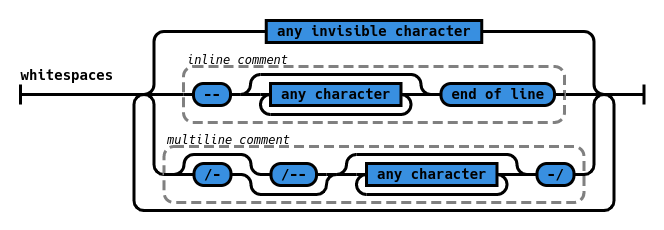
\includegraphics{zilch/lexicon/whitespaces}
		}
	}

	\caption{Whitespace lexical units.}
	\label{fig:zilch-grammar-lexical-whitespaces-grammar}
\end{figure}

\subsection{Numerical tokens}\label{subsec:zilch-grammar-lexical-numbers}

There are two kinds of numerical tokens: integers and floating points.
While floating points are always written using decimal digits, integers may be written using decimal digits, octal digits (if prefixed by \verb|0o| or \verb|0O|), hexadecimal digits (if prefixed by \verb|0x| or \verb|0X|) or binary digits (if prefixed by \verb|0b| or \verb|0B|).
A floating point number must always have digits on both sides of the dot (i.e.\ it is impossible to write \verb|0.| as in other programming languages) because it could else be mistaken with the dot syntax.

\begin{figure}[H]
	\centering

	\framebox[\textwidth][c]{
		\scalebox{.5}{
			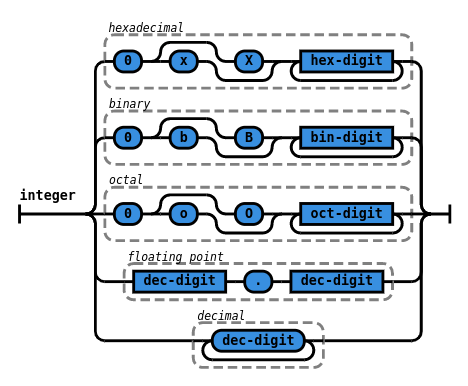
\includegraphics{zilch/lexicon/number}
		}
	}

	\caption{Numeric lexical units.}
	\label{fig:zilch-grammar-lexical-numbers-grammar}
\end{figure}

\subsection{String and character literals}\label{subsec:zilch-grammar-lexical-strings}

Strings are arrays of characters.
However, because it is tedious to write such arrays, we provide syntactic sugar to make it easier.

String literals are enclosed in double quotes \verb|"|, and character literal are enclosed in single quotes \verb|'|.
They can contain any character (both graphical and whitespaces), but some characters may be easier to type.
These basically have ``shorthands'' defined as escape sequences, each defined in Table~\ref{table:zilch-grammar-lexical-strings-escapesequences}.
Note that, while double and single quotes may be escaped, these may not necessarily be in respectively character and string literals.

Multiple string literals directly next to each other (as in \verb|"abc" "def"|) are concatenated into one (so \verb|"abcdef"|).

\begin{figure}[H]
	\centering

	\framebox[\textwidth][c]{
		\parbox{\textwidth}{
			\centering

			\scalebox{.5}{
				\includegraphics{zilch/lexicon/string}
			}
			\\
			\scalebox{.5}{
				\includegraphics{zilch/lexicon/character}
			}
		}
	}

	\caption{String and character lexical units.}
	\label{fig:zilch-grammar-lexical-strings-grammar}
\end{figure}

\begin{table}[htb]
	\begin{tabularx}{\textwidth}{*{5}{Y}}
		\toprule
		\verb|\a| & \verb|\b| & \verb|\f| & \verb|\n| & \verb|\r| \\
		\verb|\t| & \verb|\v| & \verb|\\| & \verb|\"| & \verb|\'| \\
		\bottomrule
	\end{tabularx}

	\caption{All available escape sequences.}
	\label{table:zilch-grammar-lexical-strings-escapesequences}
\end{table}

\section{Expressions}\label{sec:zilch-grammar-expressions}

Expressions are the basic building block of Zilch.
\textit{Everything} is an expression, from simple arithmetic like \texttt{3 + 6} to complex \texttt{let-in} expressions.

\subsection{Lambda abstraction}\label{subsec:zilch-grammar-expressions-lambda}

Lambda abstractions allow creating ``in-place'' anonymous functions.
For example, both following alternatives are equivalent (because the lambda abstraction does not capture anything there):\\
\inputminted{\zilchlexer}{examples/captureless-lambda-equivalence.zc}
\vspace*{\baselineskip}

\noindent However, these two are not quite equivalent:\\
\inputminted{\zilchlexer}{examples/closure-non-equivalence.zc}
\vspace*{\baselineskip}

\noindent Note that lambda abstractions cannot be recursive on their own, they need to be bound using a \texttt{def} declaration.

There is also an alternative grammar for lambda abstractions, using wildcards abstractions.
Sometimes, you have to write \verb|reduce((acc, e) -> acc + e, 0, list)|.
While functional, this is a bit ugly and can be greatly shortened.
This is why there are wildcard abstractions: it allows writing \verb|reduce(_ + _, 0, list)| which makes it cleaner looking.
\verb|_ + _| is really syntactic sugar for \texttt{($x_0$, $x_1$) -> $x_0$ + $x_1$}\footnote{Please be aware that \texttt{\_+\_} and \texttt{\_ + \_} are not actually the same entities: the former is binary operator \texttt{+} while the latter is a two parameter lambda.}.

A simple rule to convert wildcard abstractions to explicit lambda abstractions is the following: for each wildcard $\cdot_i$ in an expression \verb|e| (assuming from the left to the right), assign an unique identifier $u_i$ and replace the wildcard with it (also increment $i$). If $i \neq 0$ at the end, then replace \verb|e| with the lambda abstraction \texttt{($u_0$, \ldots, $u_i$) -> e[$\cdot_0$\textbackslash$u_0$, \ldots, $\cdot_i$\textbackslash$u_i$]}.
Some examples are given in Table~\ref{table:zilch-grammar-expressions-lambda-translatewildcard}.

\begin{figure}[H]
	\centering

	\framebox[\textwidth][c]{
		\scalebox{.5}{
			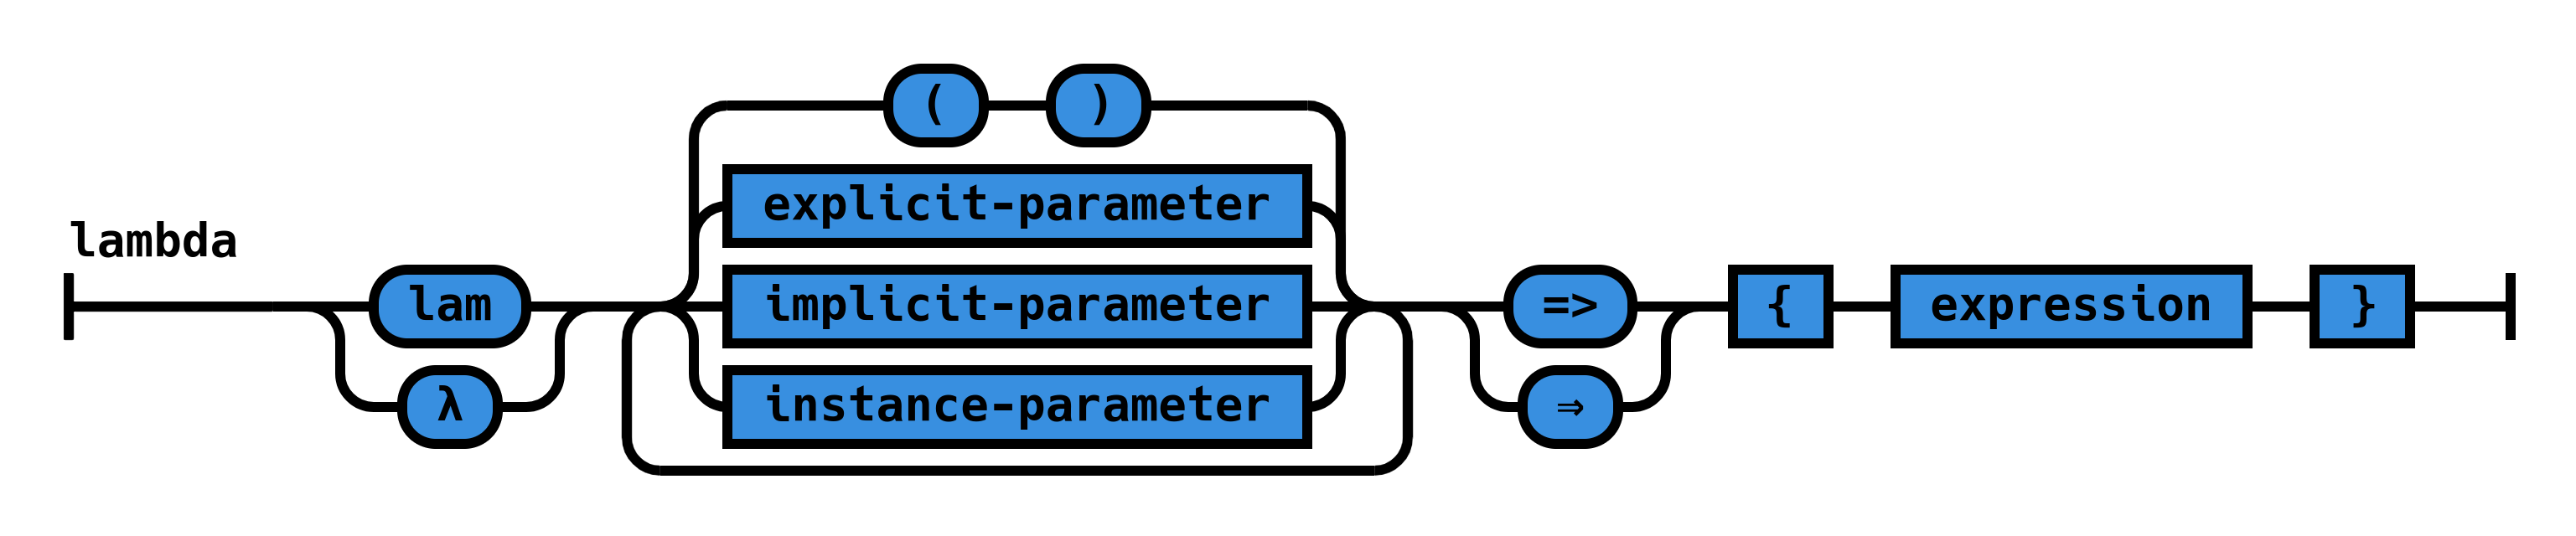
\includegraphics{zilch/expression/lambda}
		}
	}

	\caption{Grammar for lambda abstractions.}
	\label{fig:zilch-gramma-expressions-lambda-grammar}
\end{figure}

\begin{table}[htb]
	\begin{tabularx}{\textwidth}{YcY}
		\toprule
		From                    & \multirow{5}{*}{\textbf{$\rightsquigarrow$}} & To                      \\
		\midrule
		\verb|_ + 1| &                                              & \verb|(x0) -> x0 + 1| \\
		\verb|f(_)| &                                              & \verb|(x0) -> f(x0)| \\
		\verb|f(_ * 2)| &                                              & \verb|f((x0) -> x0 * 2)| \\
		\verb|f(_ * 2, _)| &                                              & \verb|(x0) -> f((x1) -> x1 * 2, x0)| \\
		\bottomrule
	\end{tabularx}

	\caption{Some examples of wildcard abstraction translation.}
	\label{table:zilch-grammar-expressions-lambda-translatewildcard}
\end{table}

\subsection{Conditional}\label{subsec:zilch-grammar-expressions-conditional}

Conditional expressions allow selecting an expression based off the value of a condition.
However, it only works as a binary selector.
If n-ary selectors are needed, chaining \texttt{if}s is the only solution.

\begin{figure}[H]
	\centering

	\framebox[\textwidth][c]{
		\scalebox{.5}{
			\includegraphics{zilch/expression/conditional}
		}
	}

	\caption{Grammar for conditional expressions.}
	\label{fig:zilch-gramma-expressions-conditional-grammar}
\end{figure}

\subsection{Let-in}\label{subsec:zilch-grammar-expressions-letin}

Let-in expressions allow binding local variables in the context of another expression.
However, it does not act the same as simply replacing the variable just like a macro because of evaluation order and potential side-effects.

\begin{figure}[H]
	\centering

	\framebox[\textwidth][c]{
		\scalebox{.5}{
			
\includegraphics{zilch/expression/let-in}
		}
	}

	\caption{Grammar for let-in blocks.}
	\label{fig:zilch-grammar-expressions-letin-grammar}
\end{figure}

\subsection{Pattern matching}\label{subsec:zilch-grammar-expressions-case}

Pattern matching is achieved through the use of a \texttt{match} expression.

\begin{figure}[H]
	\centering

	\framebox[\textwidth][c]{
		\parbox{\textwidth}{
			\centering

			\scalebox{.5}{
				\includegraphics{zilch/expression/pattern}
			}\\
			\scalebox{.5}{
				%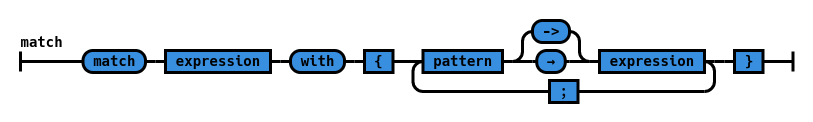
\includegraphics{zilch/expression/match}
			}
		}
	}

	\caption{Grammar for case expressions.}
	\label{fig:zilch-gramma-expressions-case-grammar}
\end{figure}

\subsection{Record literals}\label{subsec:zilch-grammar-expressions-record}

Record literals allow constructing records in the same fashion as in e.g.\ C.
The grammar uses the two terminals \verb|{{| and \verb|}}| to distinguish them from applying implicit parameters.

\begin{figure}[H]
	\centering

	\framebox[\textwidth][c]{
		\scalebox{.5}{
			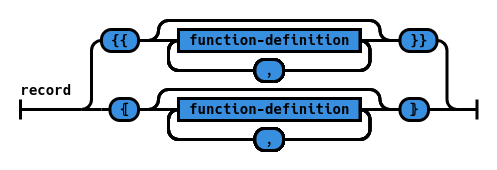
\includegraphics{zilch/expression/record}
		}
	}

	\caption{Grammar for record literals.}
	\label{fig:zilch-gramma-expressions-record-grammar}
\end{figure}

\subsection{Variables, typed holes and literals}\label{subsec:zilch-grammar-expressions-basicexpr}

\begin{figure}[H]
	\centering

	\framebox[\textwidth][c]{
		\scalebox{.5}{
			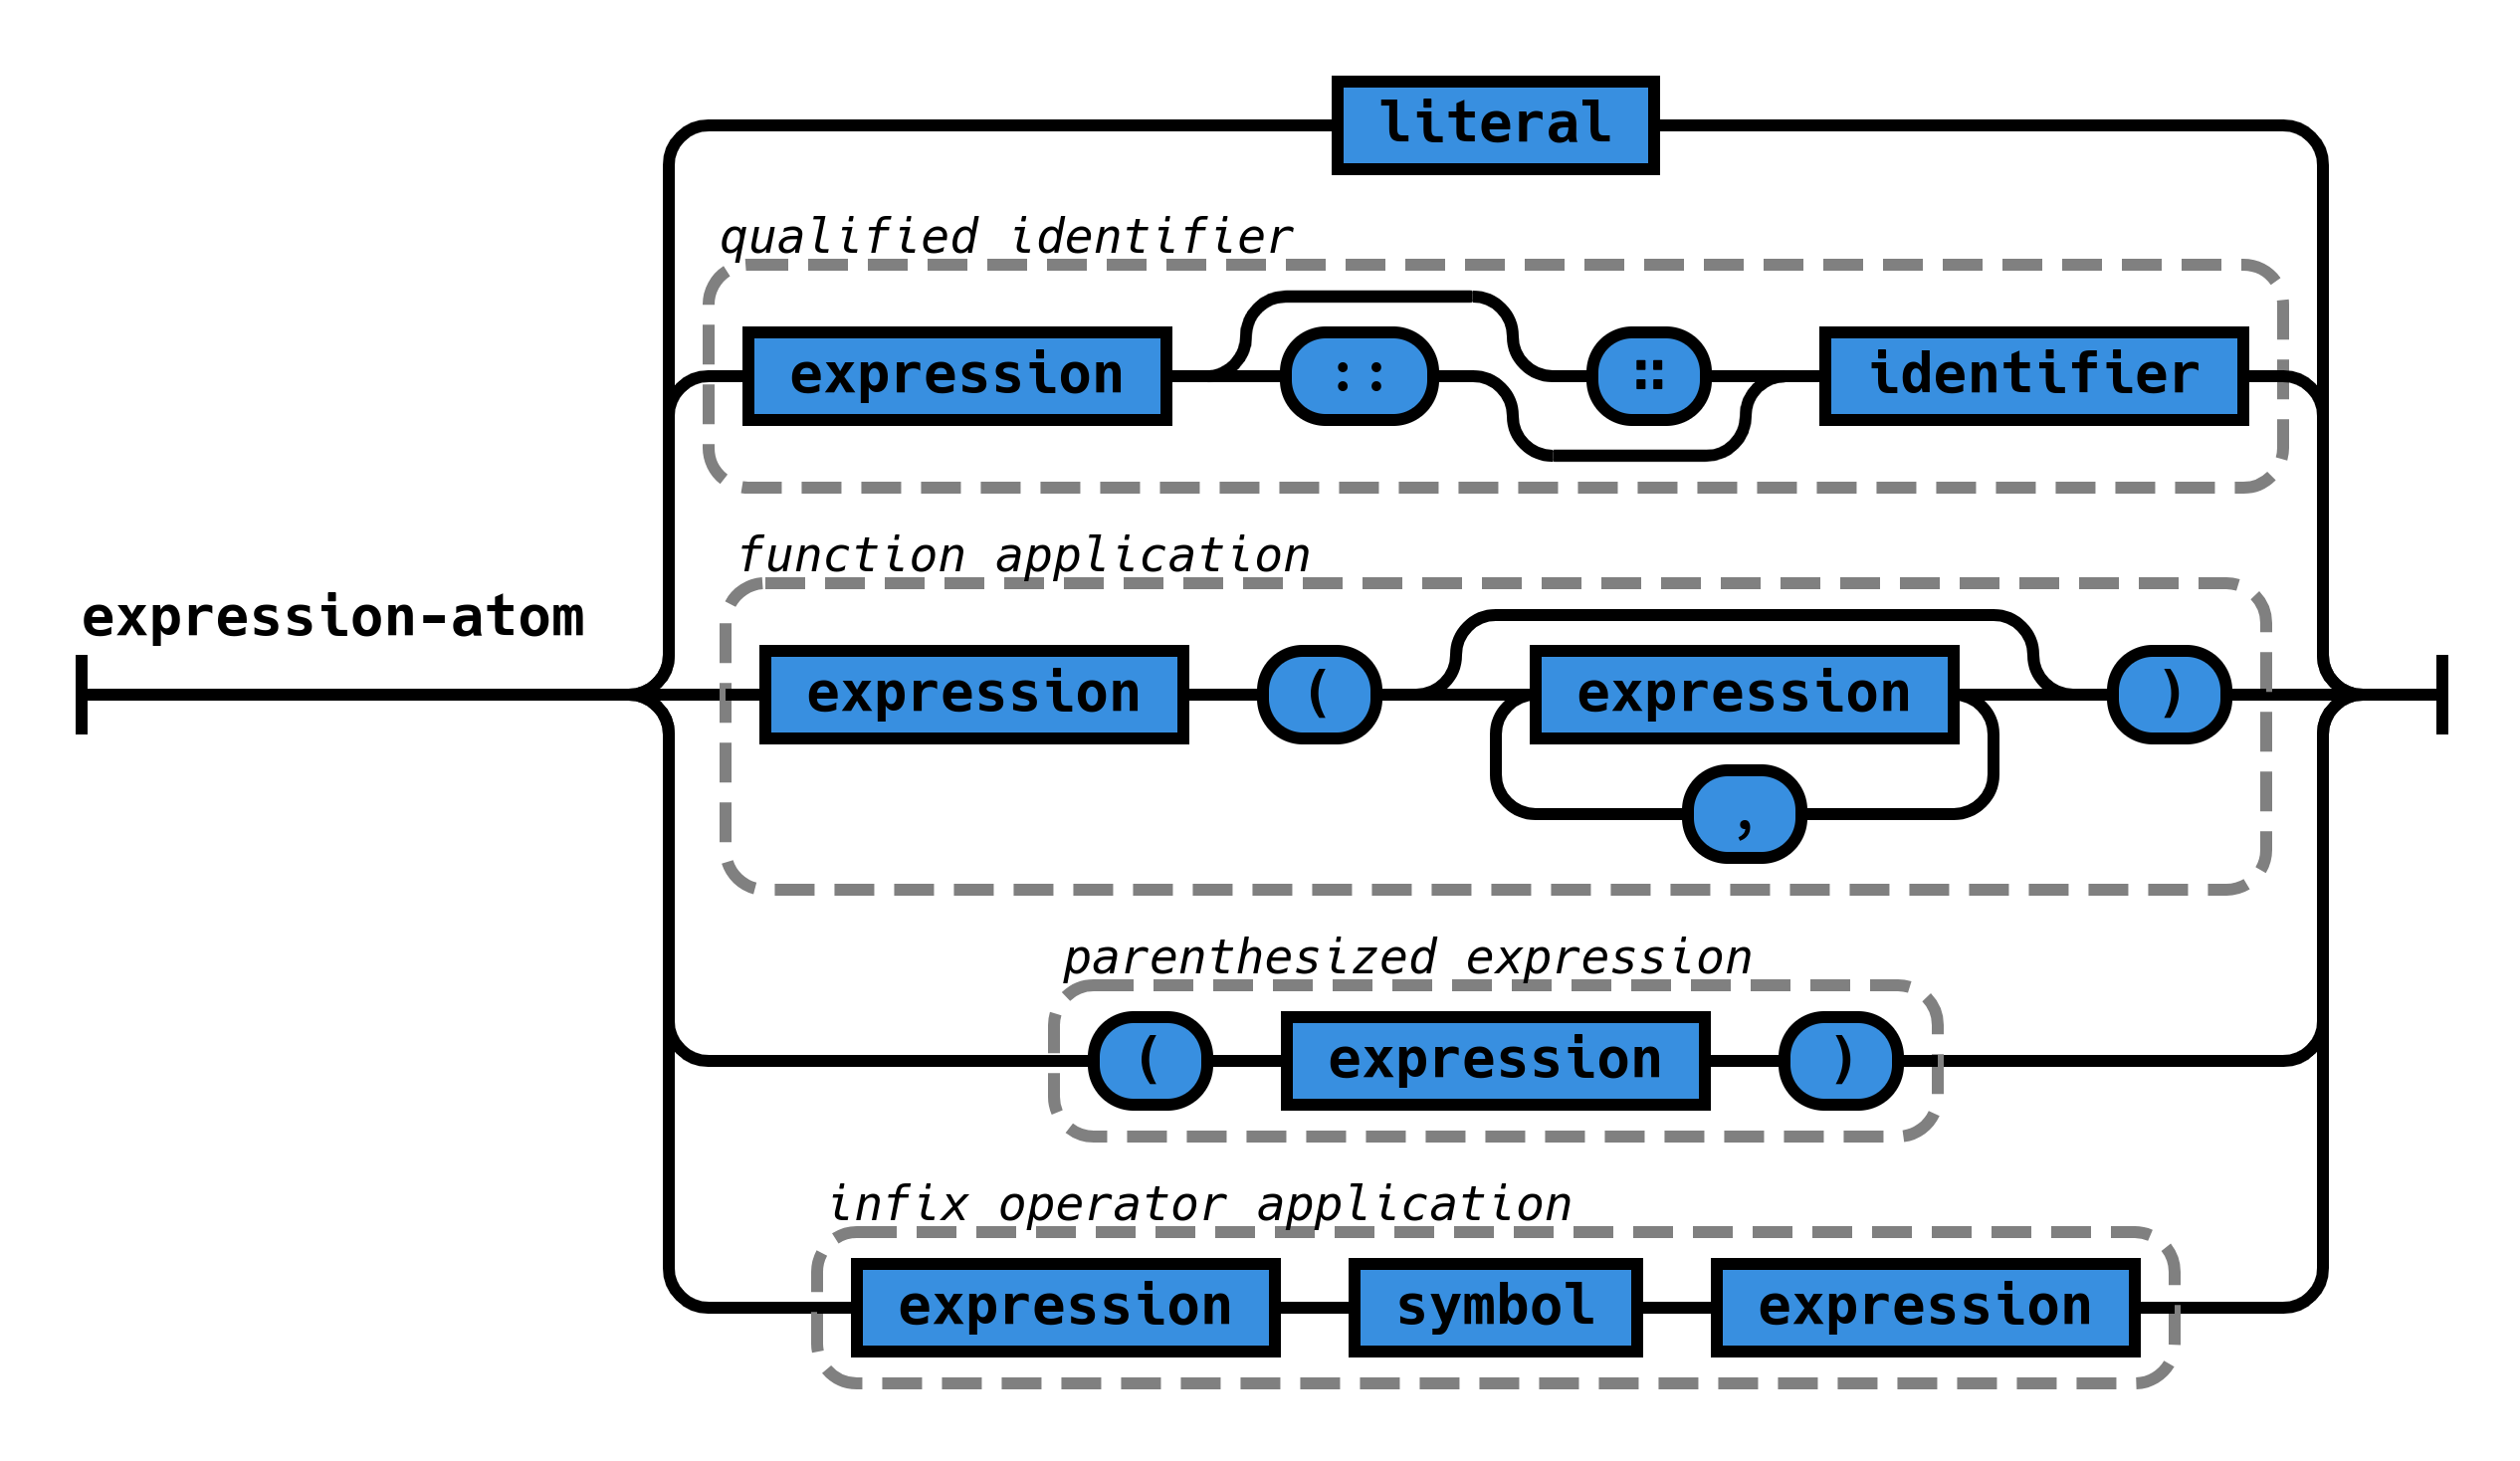
\includegraphics{zilch/expression/atom}
		}
	}

	\caption{Grammar for expression atoms.}
	\label{fig:zilch-grammar-expressions-atom-grammar}
\end{figure}

\section{Types}\label{sec:zilch-grammar-types}

Types lie at the same level as expressions, but are put in a separate section for comprehensiveness sake.
An expression \verb|e| is said to be of type \verb|t| if evaluating it yields (or at least is supposed to) any value in the set \verb|t|.

\begin{figure}[H]
	\centering

	\framebox[\textwidth][c]{
		\parbox{\textwidth}{
			\centering

			\scalebox{.5}{
				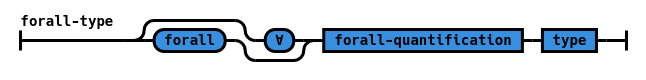
\includegraphics{zilch/types/forall}
			}\\
			\scalebox{.5}{
				\includegraphics{zilch/types/application}
			}\\
			\scalebox{.5}{
				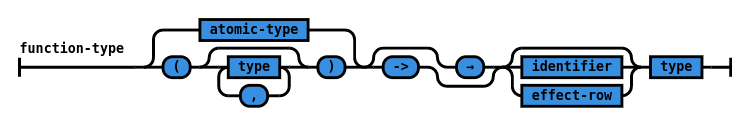
\includegraphics{zilch/types/function}
			}\\
			\scalebox{.5}{
				\includegraphics{zilch/types/builtin}
			}\\
			\scalebox{.5}{
				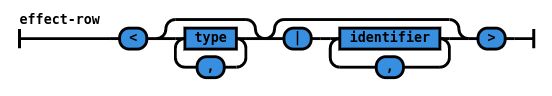
\includegraphics{zilch/types/effect-row}
			}
		}
	}

	\caption{Grammar for types.}
	\label{fig:zilch-grammar-types-grammar}
\end{figure}

Every type is also assigned a type (called ``kind'').
Kind polymorphism is not supported.

\begin{figure}[H]
	\centering

	\framebox[\textwidth][c]{
		\scalebox{.5}{
			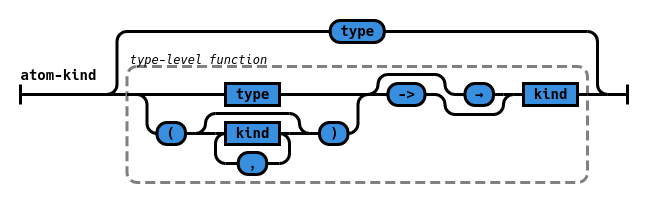
\includegraphics{zilch/types/kind}
		}
	}

	\caption{Grammar for kinds.}
	\label{fig:zilch-grammar-types-kindgrammar}
\end{figure}

\section{Declarations}\label{sec:zilch-grammar-declarations}

A Zilch module is composed of zero or more declarations.
There are 5 possible declarations:
\begin{itemize}
	\item Type class declaration
	\item Type class implementation
	\item New type definition
	\item Value definition
\end{itemize}

\noindent Each of them will be syntactically described in this section.

\subsection{Value definition}\label{subsec:zilch-grammar-declarations-value}

A function binding binds a variable to a value.
Both when the value is of a function type or of a simple value type, the binding is called a \textit{function binding}.
\vspace*{\baselineskip}

Because functions are first-class in Zilch, both function bindings defined below are completely equivalent (the lambda abstraction does not capture anything here):

\noindent\inputminted{\zilchlexer}{examples/function-value-equivalence.zc}
\vspace*{\baselineskip}

Function bindings may additionally be accompanied by \verb|where| blocks, which allow binding local variables in the scope of the expression.
This is mostly equivalent to putting those bindings at the beginning of a \verb|let-in| block:

\noindent\inputminted{\zilchlexer}{examples/function-where-let-equivalence.zc}

Note that recursive function bindings (bindingis calling themselves in their definitions) are only allowed for \textit{functions}, and must be prefixed by \verb|rec| instead of \verb|let|.

Mutable function bindings are only allowed for non-recursive value bindings (i.e. \verb|let mut x : t| is allowed (if \verb|t| is a value type) but neither \verb|rec mut x : t| nor \verb|let mut f : a -> b|).

top-level function bindings can additionnally be prefixed with special meta-attributes (described later in Section~\ref{subsec:zilch-grammar-declarations-meta}).

\begin{figure}[H]
	\centering

	\framebox[\textwidth][c]{
		\parbox{\textwidth}{
			\centering

			\scalebox{.45}{
				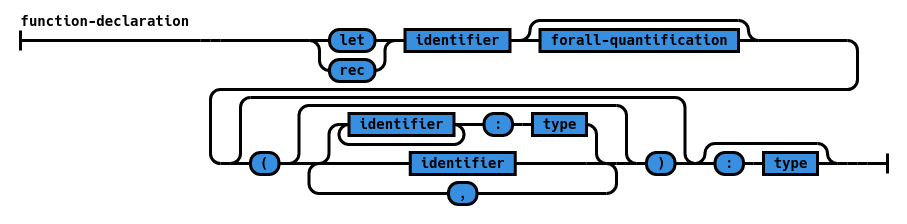
\includegraphics{zilch/toplevel/function-declaration}
			}\\
			\scalebox{.5}{
				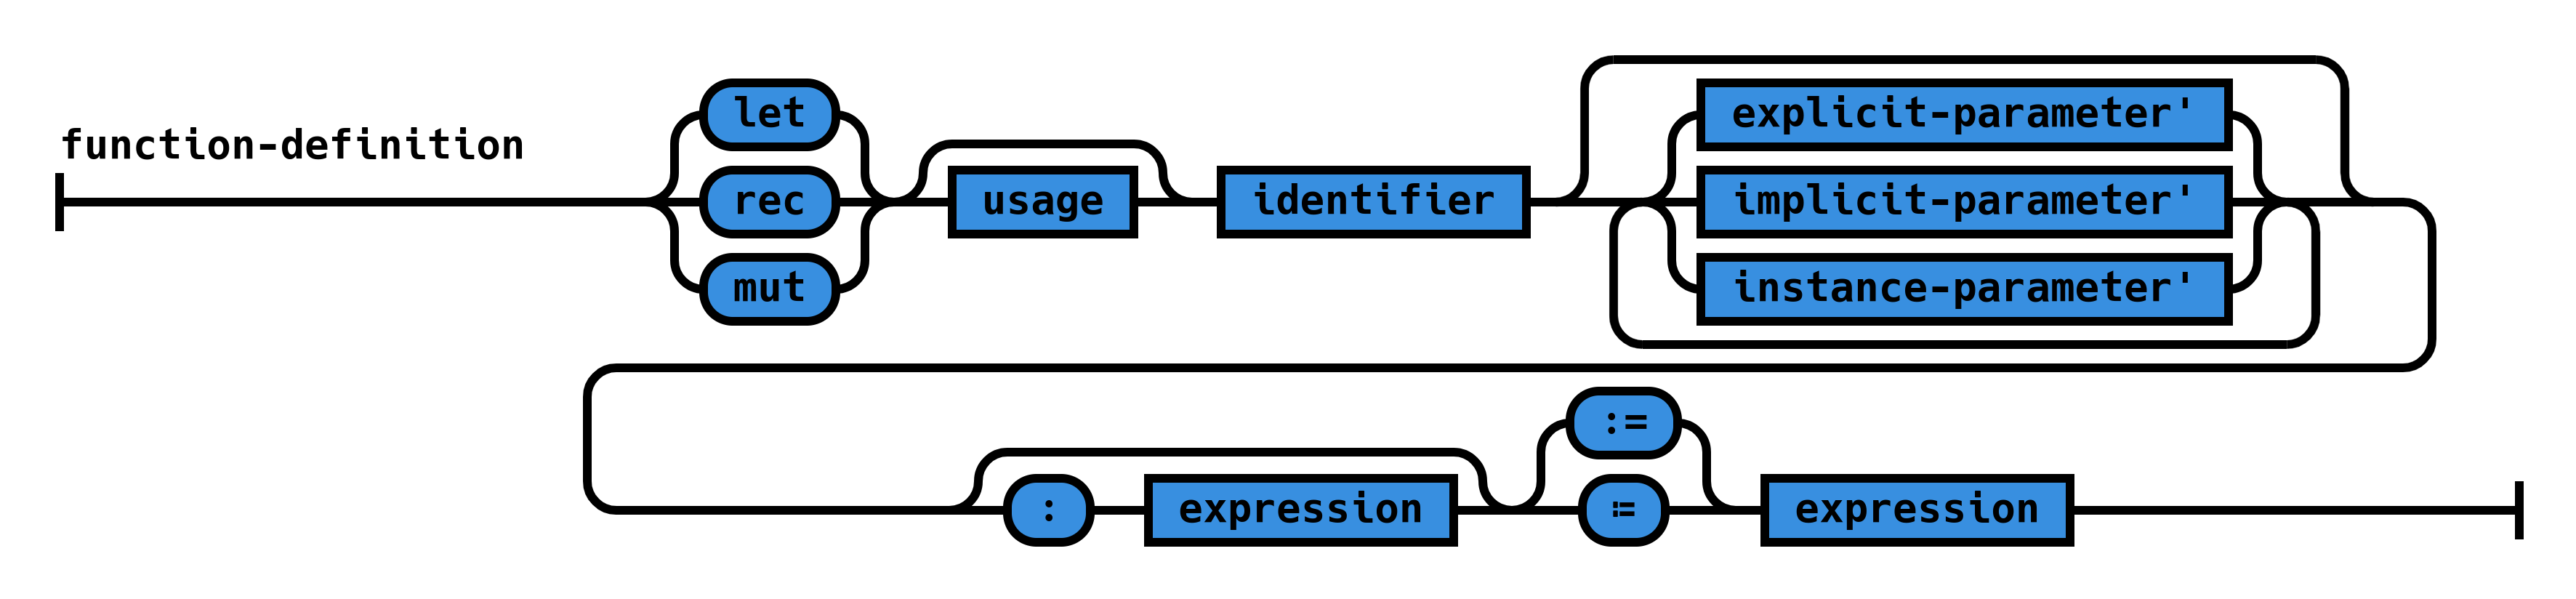
\includegraphics{zilch/toplevel/function-definition}
			}\\
			\scalebox{.45}{
				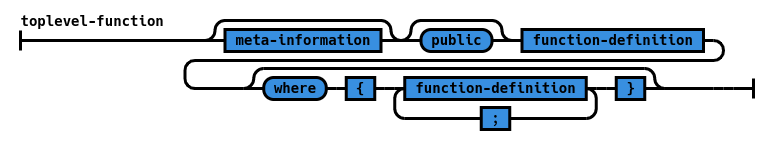
\includegraphics{zilch/toplevel/toplevel-function-definition}
			}
		}
	}

	\caption{Grammar for value declarations.}
	\label{fig:zilch-grammar-declarations-value-grammar}
\end{figure}

\subsection{New type definition}\label{subsec:zilch-grammar-declarations-type}

Sometimes, only working with primitive types is limiting.
For example, a function returning an unsigned integer may need to indicate some sort of error.

\noindent C-style programming languages use special values which are considered invalid as return values (e.g.\ $-1$).
This doesn't quite work when no return value from the return set is actually invalid, but the function is still expected to be able to indicate failure.

\noindent More evolved programming languages use exceptions, which are not integrated in Zilch.

\noindent This is where custom types come in: it is possible to define a new ``or''-type (called ``enum'' in Zilch) to represent either a return value or no return value (in the case of a failure), usually called ``\texttt{Option}'' or ``\texttt{Maybe}''.

A function may also be expected to return multiple values.
In C-style programming languages, making use of references/pointers is one way, but using structures (called ``record''s) is the way to go in Zilch.

And some other times, using a specific type is not semantically clear enough.
For example, what does a \texttt{u64} mean as input to a function?
Zilch allows defining type aliases to address this issue, leading to code more clear.

\begin{figure}[H]
	\centering

	\framebox[\textwidth][c]{
		\parbox{\textwidth}{
			\centering

			\scalebox{.5}{
				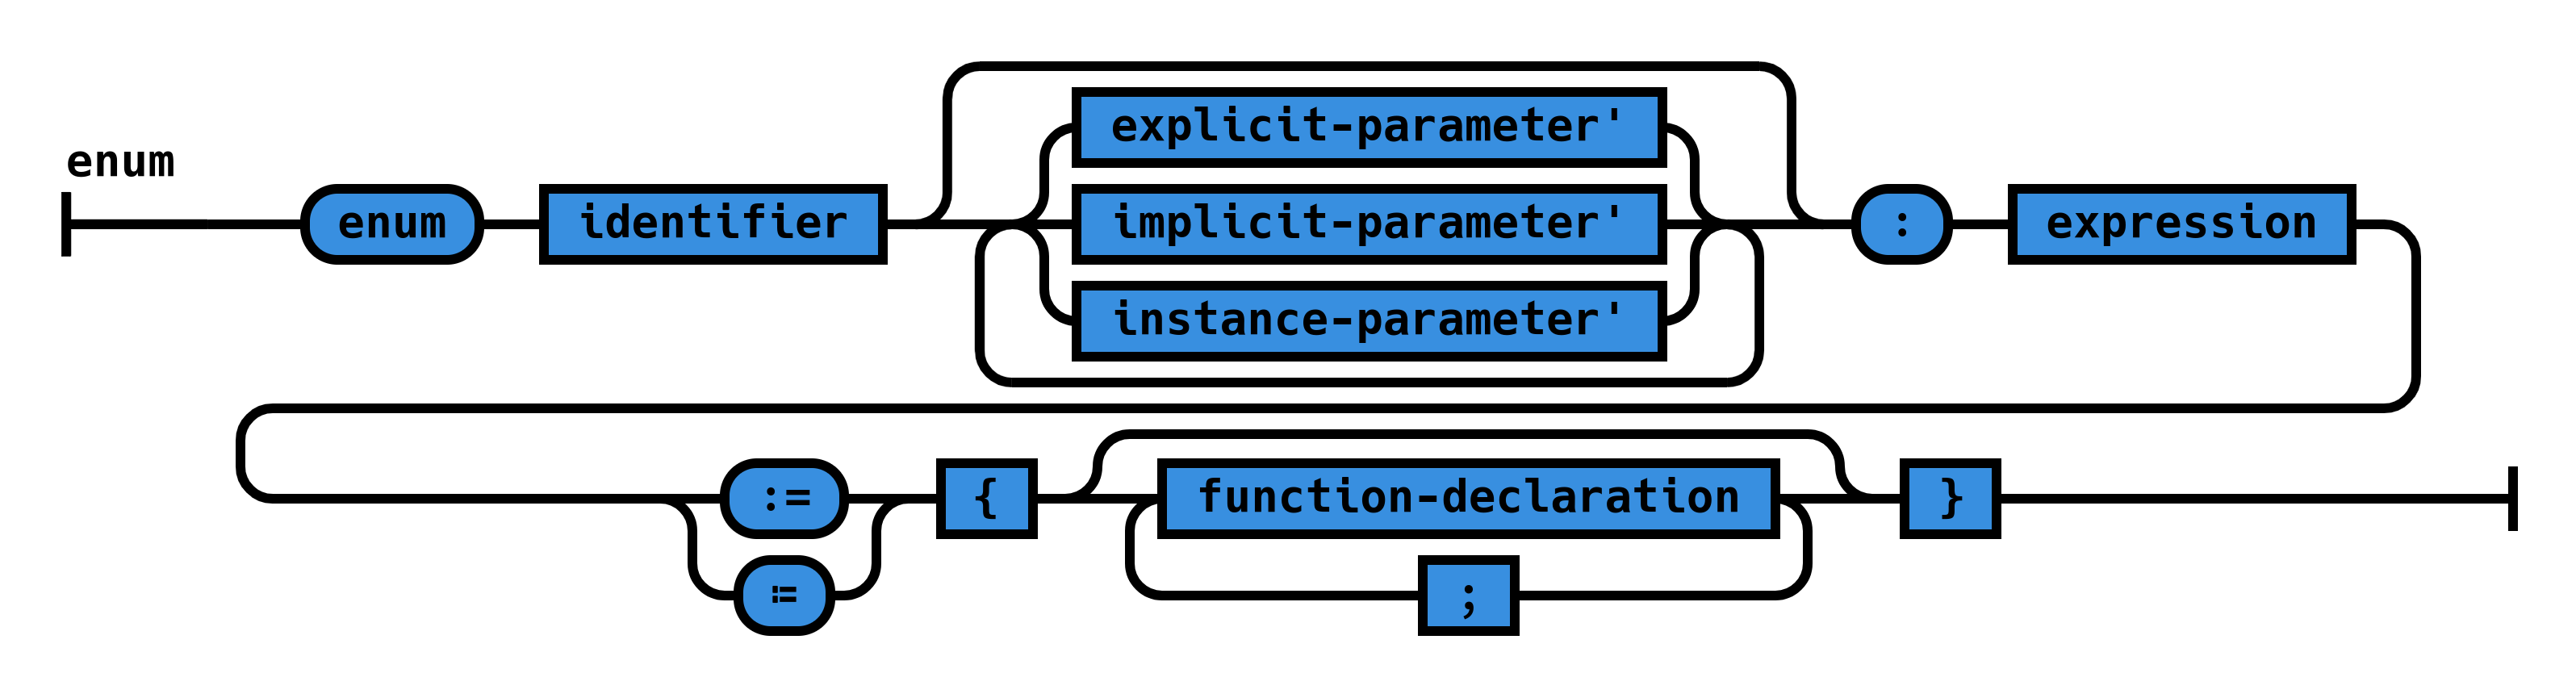
\includegraphics{zilch/toplevel/enum-definition}
			}\\
			\scalebox{.5}{
				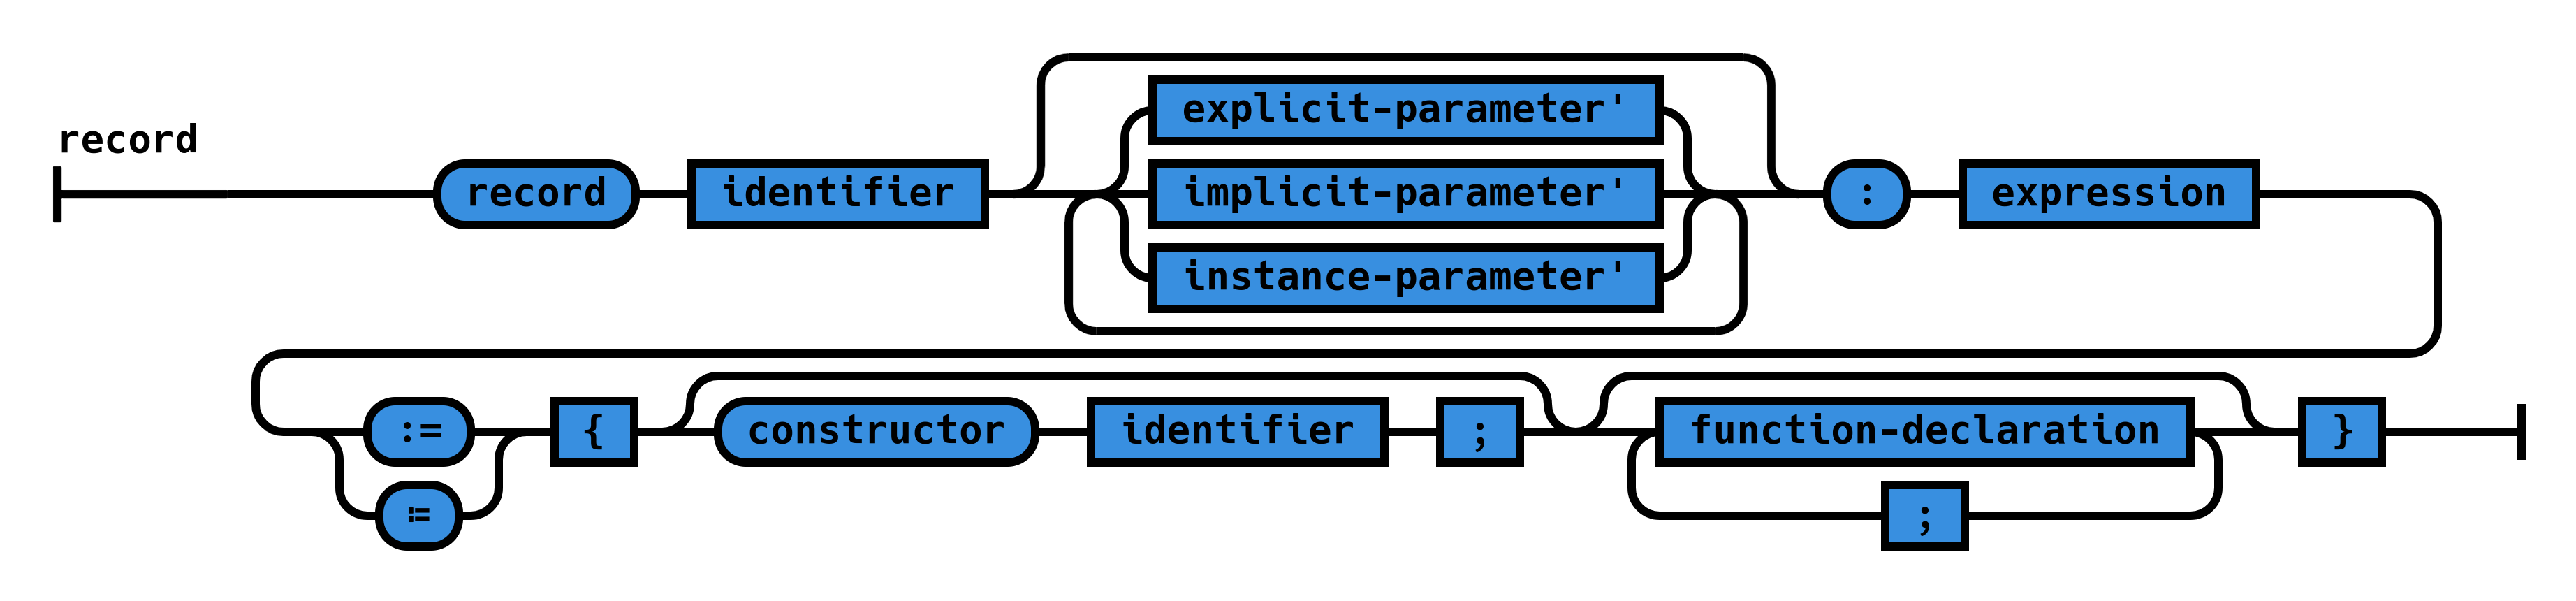
\includegraphics{zilch/toplevel/record-definition}
			}\\
			\scalebox{.5}{
				\includegraphics{zilch/toplevel/alias-definition}
			}
		}
	}

	\caption{Grammar for new type definitions.}
	\label{fig:zilch-grammar-declarations-type-grammar}
\end{figure}

\subsection{Meta-information}\label{subsec:zilch-grammar-declarations-meta}

Meta-information can be added to any top-level declaration.
They can be used for example to declare operator fixities, or add deriving clauses to auto-generate type class instances.
Any declaration accepts zero or more meta-specifiers, but each specifier is restricted as per these rules:
\begin{itemize}
	\item Fixity specifiers can only be applied to mixfix operators.
	      These are used to disambiguate expressions, and come in 5 flavors:
	      \begin{itemize}
		      \item \verb|infix <prec>|, \verb|infixr <prec>| and \verb|infixl <prec>| allow specifying the associativity (left, right or none) and precedence of infix operators (operators of the form \verb|_..._|);
	      \end{itemize}
	\item Deriving clauses can only be added to \verb|enum| and \verb|record| types;
	\item Inlining hints tell the compiler that a function may not have a huge cost, therefore can be inlined more easily;
	\item FFI imports/exports, to either retrieve or give a function defined in another compilation unit (most probably coming from another programming language like C);
	\item Default effect handlers can be added to any function binding of type \verb|{e} -> {a} -> (() -> < eff | e > a) -> e a| (meaning it consumes the effect \verb|eff| given) (implicits may be given in any order).
				These are used to remove any additional effects on the \verb|main| function without having to specify each of them.
				Note that those handlers are implicitly exported (even when not \verb|public|) and will be used transparently, but still need to be \verb|public| to be used by hand.
\end{itemize}

\begin{figure}[H]
	\centering

	\scalebox{.5}{
		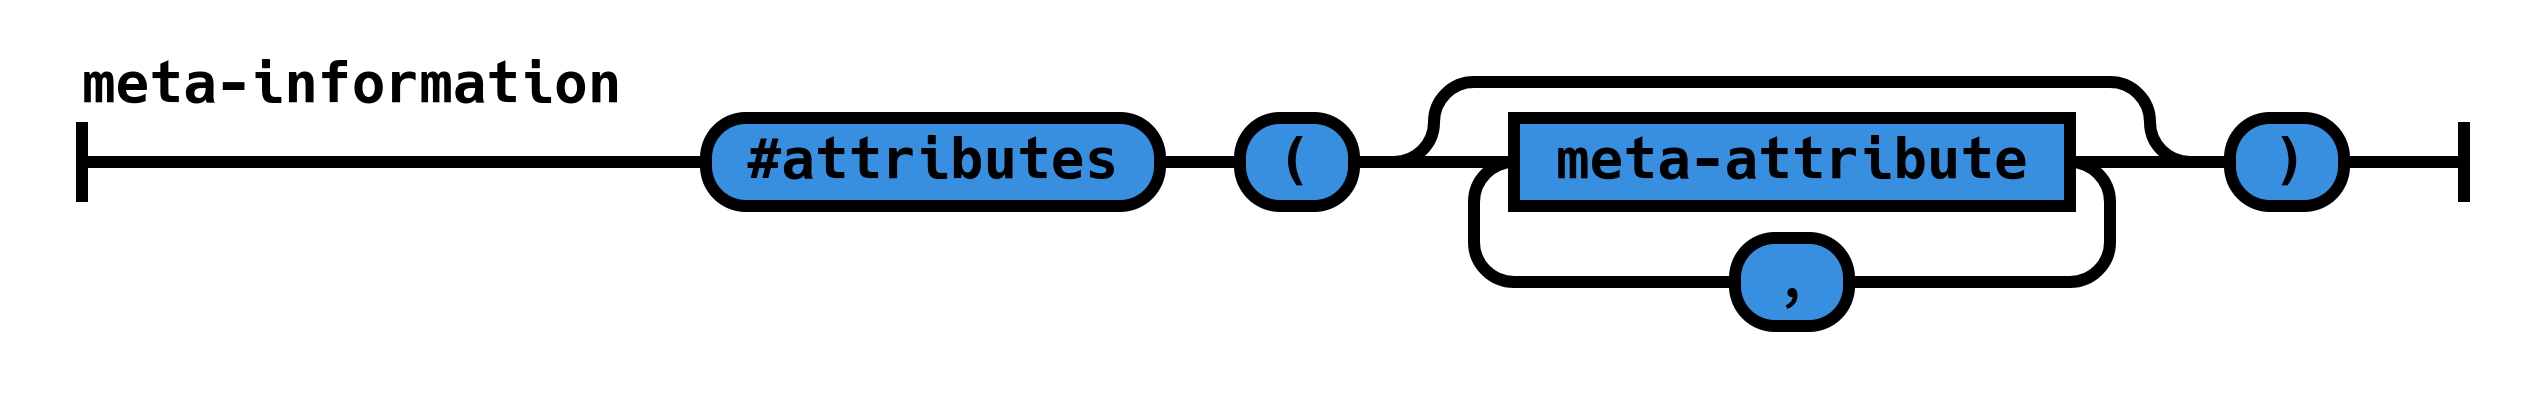
\includegraphics{zilch/toplevel/meta-information}
	}\\
	\scalebox{.5}{
		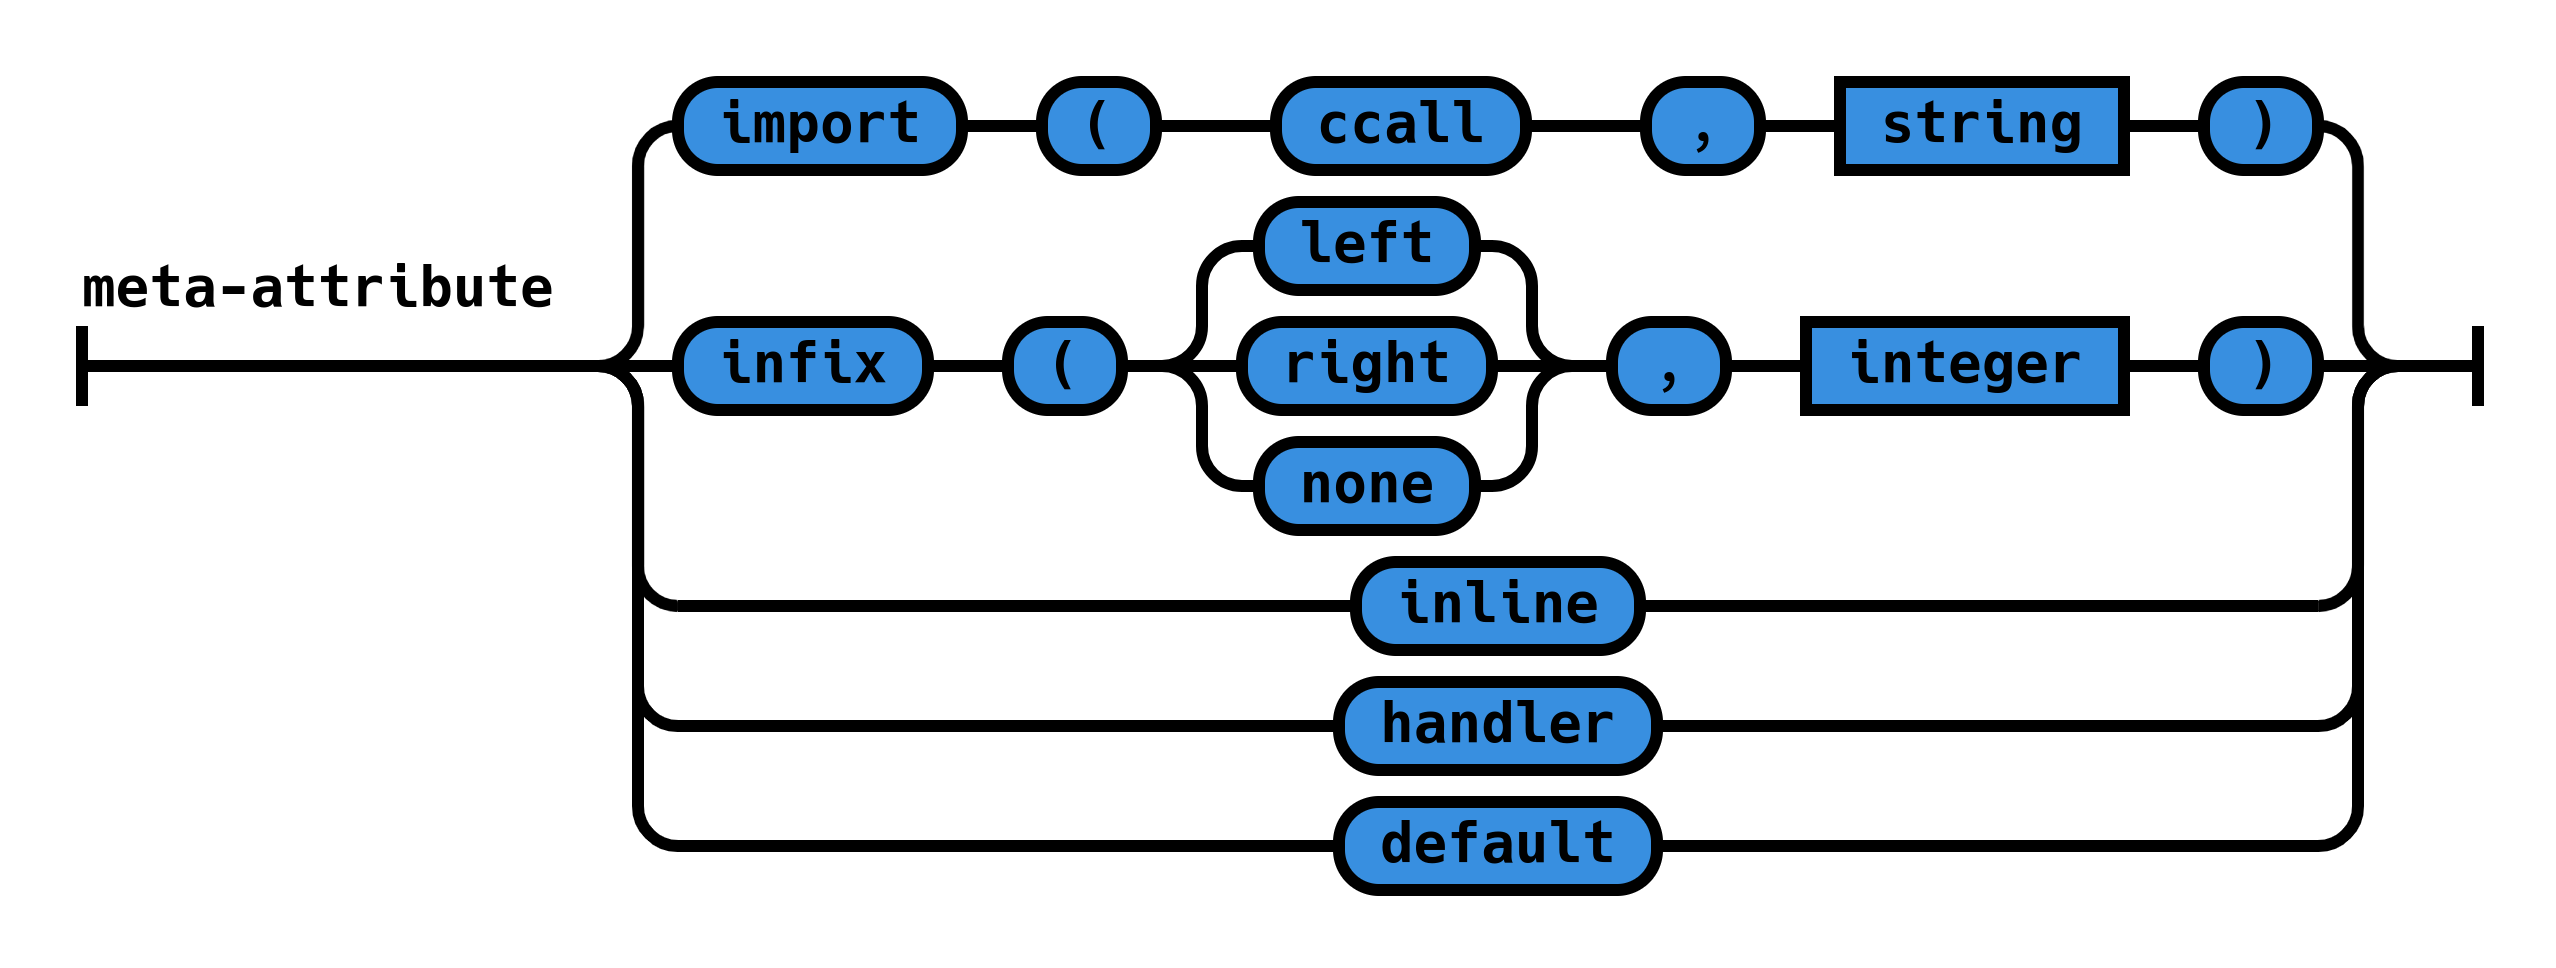
\includegraphics{zilch/toplevel/meta-specifier}
	}
	% TODO: add #[handler]

	\caption{Grammar for meta-specifiers.}
	\label{fig:zilch-grammar-declarations-meta-grammar}
\end{figure}

\section{Modules}\label{sec:zilch-grammar-modules}

Modules allow grouping functions and types that are related to each other under a common namespace.
In Zilch, modules provide grouping, importing and visibility restrictions.

A Zilch module is declared according to the name and position of the file in the include path.
For example, if a file is named \verb|Internal.zc| in the directory \verb|Data/Something/A|, then it exports a module \verb|Data::Something::A::Internal|.

It can contain, in this order, many (possibly none) \texttt{import} statements (see Figure~\ref{fig:zilch-grammar-modules-importgrammar}) and any number of declarations as described in Section~\ref{sec:zilch-grammar-declarations}~``\nameref{sec:zilch-grammar-declarations}''.

A module $A$ may export another module $B$, meaning that anything imported from $B$ into $A$'s scope is exported by $A$.
If a plain function is aliased\footnote{Infix operators cannot be aliased because it would lead to many syntactical problems.} from the import of $B$ in $A$, the new name is exported by $A$ instead of the old one.
Operator fixities are exported only if their corresponding operators are also exported.
All imports are qualified, unless when \verb|open|ed.

\begin{figure}[H]
	\centering

	\scalebox{.5}{
		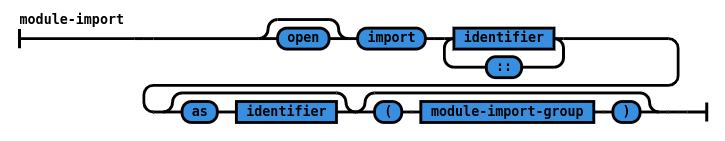
\includegraphics{zilch/modules/import}
	}\\
	\scalebox{.5}{
		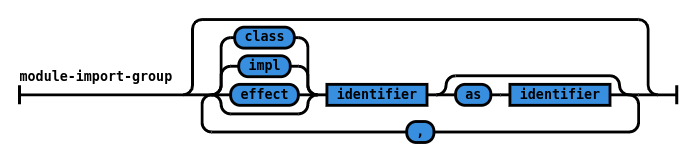
\includegraphics{zilch/modules/import-group}
	}

	\caption{Grammar for import statements.}
	\label{fig:zilch-grammar-modules-importgrammar}
\end{figure}

\chapter{Static semantics}\label{chap:zilch-staticsem}

Zilch is statically and strongly typed, meaning that types of expressions are checked at compile-time, and no implicit conversion are performed.
It also is type-infered, so there is no need to write the exact type of a function (unless in specific ambiguous states, e.g. with constraints).

The type system of Zilch, used to type expressions and types is described in this chapter using typing rules, each accompanied by an informal description.
Some sections may not contain typing rules just for the sake of simplicity: an informal description will be more descriptive in those cases.

\section{Types of types}\label{sec:zilch-staticsem-types}

In Zilch, not only expressions have types, but types also do (in such case, types of types are called “kinds” and we will refer to that in the next part).
While this may sound a little bit complex, it in fact allows easily solving a few problems happening in some of other programming languages allowing generic programming:
\begin{itemize}
	\item A type may be passed partially applied to a function or a type.
	\item Type constraints live as inhabitants of other sets of types.
	      As such, constraints cannot be passed in place of other types, which would imply weird type system behaviours.
	\item A partially applied type (in opposition to a fully applied type, called a ``concrete kind'') cannot be given to a function requiring a concrete type.
\end{itemize}

Types of types are mainly organized in 4 categories:
\begin{itemize}
	\item Concrete types, which are denoted as \verb|type| in Zilch, are types which are fully applied to arguments.
	\item Partially applied types (also called ``type constructors'') can only be applied to more arguments, but may yield any kind of type.
	      Just like functions at the expression level, type constructors are written using the arrow syntax \verb|_->_|.
	\item Type constraints are specific kinds of types allowing to specify bounds on types they depend on.
	      The set of type constraints is called \verb|constraint|.
	\item Effect types are special kinds of types which are only allowed to specify possible effects when computing a function.
	      Such types are grouped under the \verb|effect| kind.
\end{itemize}

Below are described the main inference rules about type kinds.

\begin{figure}[H]
	\centering
	\begin{prooftree}
		\hypo{\tau\ \text{is atomic}}
		\infer1[\textsc{[Concrete]}]{\Delta\Vdash\tau : \text{type}}
	\end{prooftree}
	\hspace{3em}
	\begin{prooftree}
		\hypo{\Delta\Vdash\tau : \kappa\to\kappa^\prime}
		\hypo{\Delta\Vdash x : \kappa}
		\infer2[\textsc{[Apply]}]{\Delta\Vdash \tau\ x : \kappa^\prime}
	\end{prooftree}
	\\\vspace{\baselineskip}
	\begin{prooftree}
		\infer0[\textsc{[Var]}]{\Gamma,\tau : \kappa;\Delta\Vdash\tau : \kappa}
	\end{prooftree}

	\caption{Typing rules for types of types.}
	\label{fig:zilch-staticsem-types-typerule}
\end{figure}

\section{Types of expressions}\label{sec:zilch-staticsem-exprs}

\subsection{Lambda abstractions}\label{subsec:zilch-staticsem-exprs-lambda}

Typing rules are not described for expression holes (also called “anonymous lambdas” earlier) because they are syntactically equivalent to explicit lambdas.
The same rules therefore apply to expression holes.

\begin{figure}[H]
	\centering
	\begin{prooftree}
		\hypo{\Gamma,x_1 : \nu_1, \ldots,x_n : \nu_n;\Delta\vdash e : \tau\vert\epsilon}
		\infer1[\textsc{[Lam]}]{\Gamma;\Delta\vdash \text{lam}(x_1,\ldots,x_n)\to e : (\nu_1, \ldots, \nu_n)\to \epsilon\ \tau\vert\epsilon^\prime}
	\end{prooftree}

	\caption{Typing rule for lambda expressions.}
	\label{fig:zilch-staticsem-exprs-lambda-typerule}
\end{figure}

The expression $e$ in the above type rules is assumed to have the parameters $x_1$ to $x_n$ in scope, else it will not be able to use them.
As for the effects, because the body of a lambda is not evaluated at the point it is defined, any effect that it would produce is instead transferred
in the type of the lambda for them to be propagated to the call site (see the typing rules of function application).
If it produces no effect (i.e. it is a pure/total expression), $\epsilon$ is $\langle\rangle$.

Note that on its own, creating a new lambda does not produce any effect.
But because we want to be able to use lambda expressions in contexts requiring effects, creating a new lambda yields any effect.
This can also be simulated by requiring that the empty effect $\langle\rangle$ be a subtype of any effect.

\subsection{Variables, typed holes and literals}\label{subsec:zilch-staticsem-exprs-vars}

\begin{figure}[H]
	\centering

	\begin{prooftree}
		\infer0[\textsc{[Var]}]{\Gamma, x : \tau;\Delta\vdash x : \tau\vert\epsilon}
	\end{prooftree}
	\hspace{3em}
	\begin{prooftree}
		\infer0[\textsc{[Hole]}]{\Gamma;\Delta\vdash \cdot : \tau\vert\epsilon}
	\end{prooftree}
	\\\vspace{\baselineskip}
	\begin{prooftree}
		\hypo{\tau\in\{\text{u8}, \text{u16}, \text{u32}, \text{u64}\}}
		\hypo{c\ \text{is an integer literal}}
		\infer2[\textsc{[Nat]}]{\Gamma;\Delta\vdash c : \tau\vert\epsilon}
	\end{prooftree}
	\\\vspace{\baselineskip}
	\begin{prooftree}
		\hypo{c\ \text{is a character literal}}
		\infer1[\textsc{[Char]}]{\Gamma;\Delta\vdash c : \text{char}\vert\epsilon}
	\end{prooftree}

	\caption{Typing rules for variables, typed holes and literals.}
	\label{fig:zilch-staticsem-exprs-vars-typerule}
\end{figure}

\section{Module semantics}\label{sec:zilch-staticsem-modules}

Let $I$ be a set of paths denoted as $\{ p_1, p_2, \ldots, p_n \}$ called the ``include path''.
Multiple relative paths referencing the same directory (e.g. \verb|../dir| and \verb|.|, assuming the current working directory is called \verb|dir|) are considered equal.

A Zilch module is identified from one of the roots in the include path.
For example, a file \verb|src/Language/X/Parser.zc| with the include path $\{ \text{src} \}$ will have \verb|Language::X::Parser| as a module name.

When importing a module into the current scope, several cases may arise:
\begin{itemize}
	\item The module name does not correspond to a file accessible from the include path.
	      In such case, an error must be thrown and compilation must be stopped.
	\item The module name corresponds to multiple files in the include path.
	      Handling this is left unspecified as several options are available.
	\item The module name corresponds to only one file in the include path.
\end{itemize}

Imports are qualified by default.
This means that all imports do not populate the current scope, unless explicitly opened.
Imports can also be aliased, where an aliased qualified import simply populates another name.
When unqualified, an alias provides a qualified way of accessing to the module's identifiers in case of scope conflict (when two imported modules have a common identifier).

Imported identifiers can also be aliased locally, only if they do not refer to operators.

Identifiers are separated by level, meaning importing the name (and definition) of, for example, an effect needs to be explicitly stated.
There are 4 levels:
\begin{itemize}
	\item The \verb|class| level, used to import type classes and their members in the current scope.
	\item The \verb|effect| level, importing effect names as well as their members.
	\item The \verb|impl| level, which locally imports a given typeclass implementation (Note that the typeclass needs to be in scoped).
	\item The default level, used to import functions, global variables and types.
\end{itemize}


Module exports follow the same rules, where not specifying which identifiers to export means that nothing is exported by the module by default.
